% % % Set the style for this file:
\pagestyle{standard}

% % % Beginning of the chapter
\chapter{Infrared thermograms analysis}\label{chapter3}

	% % % Set the style for the first page:
	\thispagestyle{chapter-first-page}

	\section{Factors affecting the IR measurements.}\label{section3.1}
	
		When we take an IR picture of any object at room temperature, for instance, we intuitively expect the entire image to be of only one color (corresponding to the ambient temperature). However, this is rarely the case. There  are several factors that can make the IR temperature readings to move away from the real values, the most important are:
		
		\begin{enumerate}[label={\arabic*)}]
			\item Different emissivity values of the objects in the image.
			\item Reflectivity and Transmissivity of the object.
			\item Spectral Response Function of the IR camera in the wavelength range in which it operates.
			\item Ambient conditions. Apparent reflected temperature.
			\item Viewing angle of the IR camera with respect to the object.
		\end{enumerate}
		
		To understand how all this factors come into play we can imagine the following situation (Figure \ref{fig3.1}).  Let's assume that we have a target which is placed in front of a generic IR sensor. We are interested in measure the amount of radiation coming from the target due to emission alone, since this will be the only measure of the “real” temperature of our object. Form Equations \ref{eq1.1} and \ref{eq1.4} we can estimate the amount of emitted IR radiation as: 
		
		\begin{equation}\label{eq3.1}
			\varepsilon(\lambda,T) \cdot N_{b}(\lambda,T)
		\end{equation}	
		
		Here $T$ is the actual (real) temperature of the target. In addition, we will have two more contributions to the amount of IR radiation flying in the direction of the sensor. This other contributions are produced by additional sources of heat. 
		The first is the amount of radiation coming from external heat sources that is reflected in the target surface. This contribution is given by:
		
		\begin{equation}\label{eq3.2}
			\rho(\lambda,T) \cdot N_{b}(\lambda,T_{r})
		\end{equation}	
	
		Where $T_{r}$ is the \textit{apparent reflected temperature} of the target surface. This is an irreducible source of IR background, even with an isolated thermal chamber, and is therefore always present in the estimation of the real surface temperature. In this sense, we can regard the interior walls of the isolation chamber (and all other equipment inside) as "external" heat sources and, as the temperature of such objects should be close to the room temperature, this apparent reflected temperature is often taken as the ambient temperature. We will discuss further on this temperature and its estimation method in the next paragraph.
		The second source of additional IR radiation is that part of the radiation coming from a heat source behind the target that is transmitted through the target itself. This contribution is determined as:
		
		\begin{equation}\label{eq3.3}
			\tau(\lambda,T) \cdot N_{b}(\lambda,T_{t})
		\end{equation}	
		
		Where $T_{t}$ is the \textit{apparent transmitted temperature}. This source of IR background can be avoided by place the target in a thermal enclosure (chamber), leaving all external heat sources outside. However, for complex objects (as the Petal) composed by layers of different materials, this factor can appear if, for example, the surface material (facing the IR sensor) is somewhat transmissive and the heat from other layers reaches them and passes through.
		
		\begin{figure}[ht!]
			\centering
			\captionsetup{justification=centering,margin=2cm}
			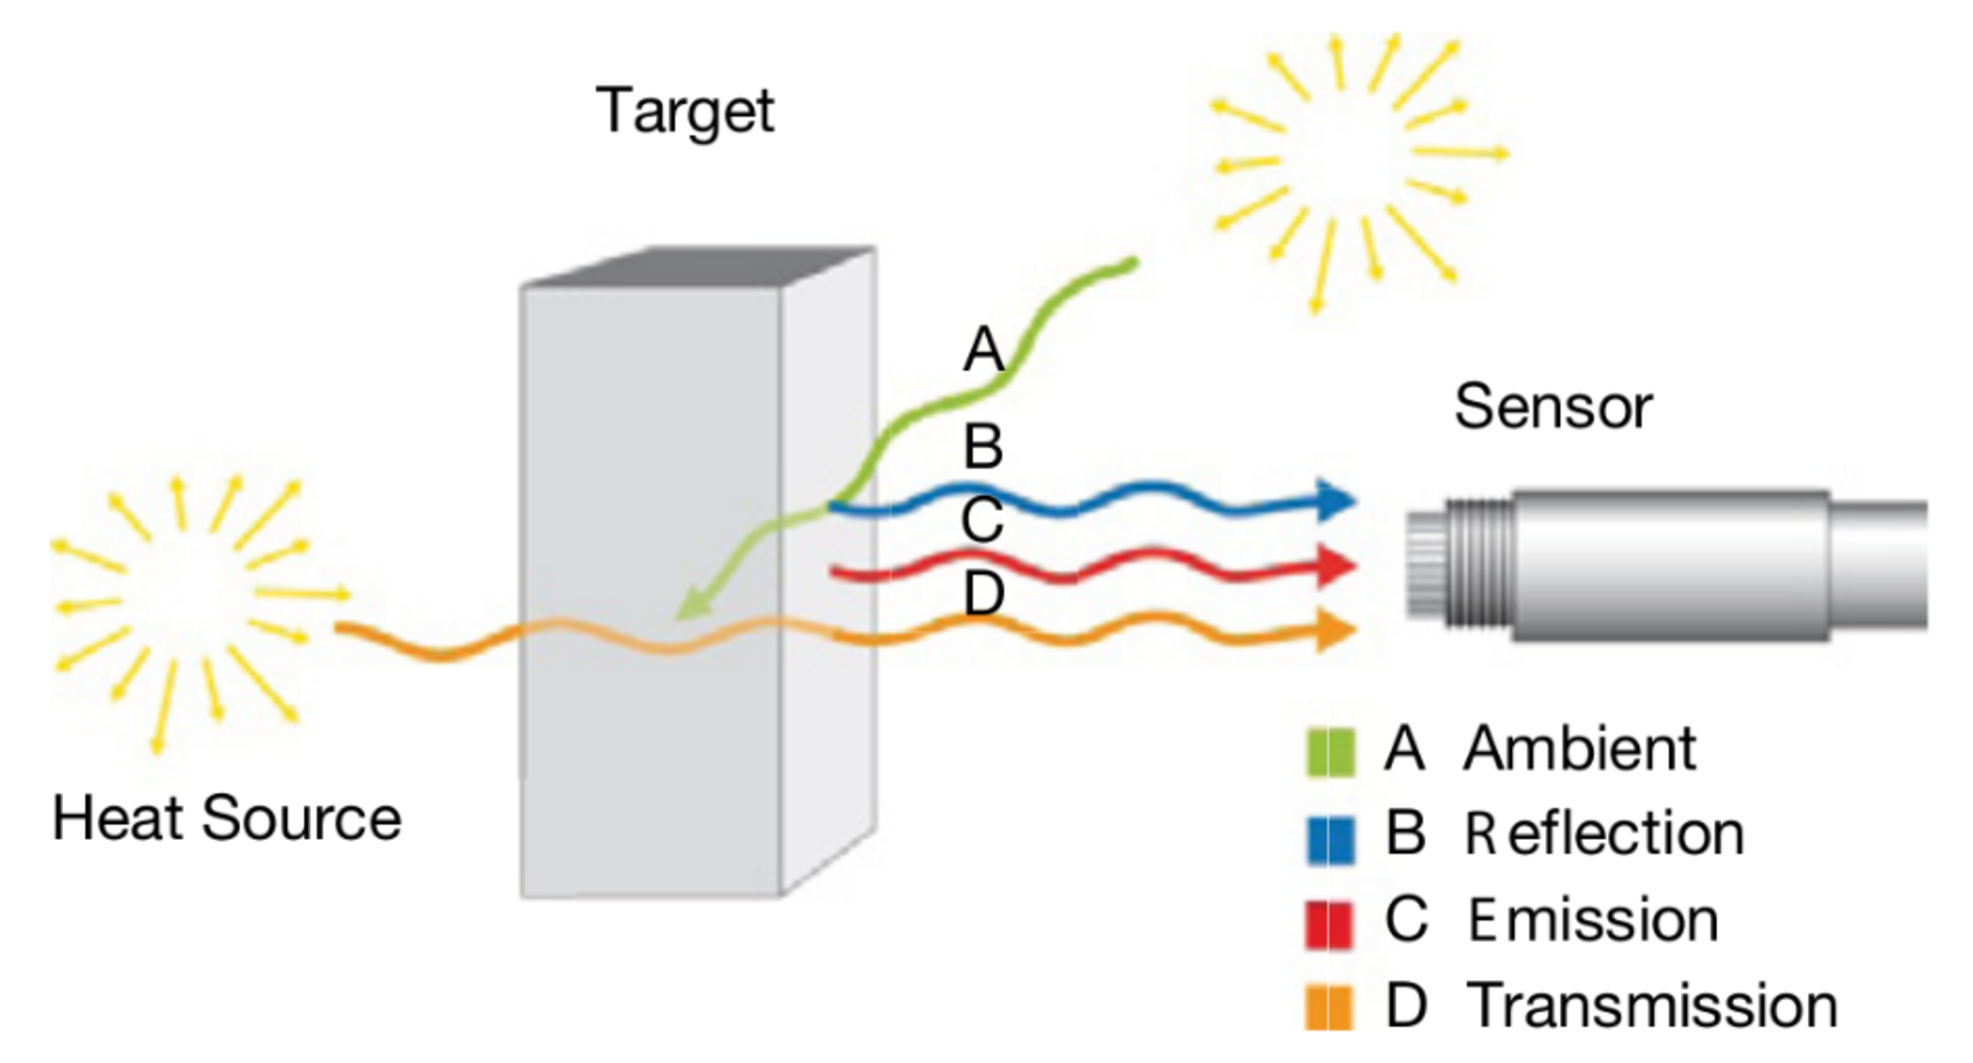
\includegraphics[scale=0.30]{Figures/Chapter03/SchematicsOfIRRadiation.pdf}
			\caption{Schematics of the IR radiation interaction with a target surface: (A) radiation from an external source being partially absorbed by the target, (B) part of the radiation from A which is reflected in the direction of the IR camera, (C) thermal  radiation emitted from the target and (D) external source radiation transmitted through the target.}\label{fig3.1}
		\end{figure}
		
		The combination of all three of this factors is then the total amount of IR radiation emanating from the target surface per unit of time and area. Neglecting the transmission component, this amount is:
		
		\begin{equation}\label{eq3.4}
			N_{total}(\lambda,T)=\varepsilon(\lambda,T) \cdot N_{b}(\lambda,T)+ [1- \varepsilon(\lambda,T)] \cdot N_{b}(\lambda,T_{r})
		\end{equation}	
		
		Where we have used Equation \ref{eq1.7} to express everything in terms of emissivity. If we also consider that this $N_{total}(\lambda,T)$ is not attenuated in the air path to the IR sensor then the emissive power registered by the sensor is:
		
		\begin{equation}\label{eq3.5}
			N_{meas}(\lambda,T)= R(\lambda) \cdot N_{total}(\lambda,T)
		\end{equation}	
		
		Where $R(\lambda)$ is the sensor's \textit{Spectral Response Function}, also known as Filter Function, accounting for the fact that the sensor is intrinsically not 100\% efficient in processing the incoming spectral power nor in the entire wavelength spectrum. As mentioned in Chapter 2, our IR camera is sensitive only in the spectral range from 7.5 $\mu$m to 14 $\mu$m, but even in that range it's also not 100\% sensitive to the incoming radiation. 
		To obtain then the total (for all wavelengths) signal processed by the IR sensor we have to integrate Equation \ref{eq3.5} over the wavelength range that our sensor is sensitive to (from $\lambda_{1}$=7.5 $\mu$m to $\lambda_{1}$=14 $\mu$m):
		
		\begin{equation}\label{eq3.6}
			N_{meas}(T)= \int_{\lambda_{1}}^{\lambda_{2}} N_{meas}(\lambda,T) d\lambda = \int_{\lambda_{1}}^{\lambda_{2}} R(\lambda) \cdot N_{total}(\lambda,T) d\lambda
		\end{equation}		
		
		\begin{equation}\label{eq3.7}
			N_{meas}(T)= \int_{\lambda_{1}}^{\lambda_{2}} R(\lambda) \cdot \varepsilon(\lambda,T) \cdot N_{b}(\lambda,T) d\lambda + \int_{\lambda_{1}}^{\lambda_{2}} R(\lambda) \cdot [1- \varepsilon(\lambda,T)] \cdot N_{b}(\lambda,T_{r}) d\lambda
		\end{equation}	
		
		As we don't know the functional form of $R(\lambda)$ or $\varepsilon(\lambda,T)$ we can come around this by applying the integral mean value theorem and use their average instead, as mentioned in Chapter 1. Since both $R(\lambda)$ and $\varepsilon(\lambda,T)$ should be slow-varying functions of the wavelength, there must be certain value $\xi\in [\lambda_{1},\lambda_{2}]$ such that we can express then Equation \ref{eq3.7} as:
		
		\begin{equation}\label{eq3.8}
			N_{meas}(T)= R(\xi) \cdot \varepsilon(\xi,T) \cdot \int_{\lambda_{1}}^{\lambda_{2}} N_{b}(\lambda,T) d\lambda + R(\xi) \cdot [1- \varepsilon(\xi,T)] \cdot \int_{\lambda_{1}}^{\lambda_{2}} N_{b}(\lambda,T_{r}) d\lambda
		\end{equation}	
		
		\begin{equation}\label{eq3.9}
			N_{meas}(T)= R \cdot \bar{\varepsilon} \cdot I_{1}(T) + R \cdot [1- \bar{\varepsilon}] \cdot I_{2}(T_{r})
		\end{equation}
		
		Where $I_{1}(T)$ and $I_{2}(T)$ we can calculate numerically:
		
		\begin{equation}\label{eq3.10}
			I_{1}(T)=\int_{\lambda_{1}}^{\lambda_{2}} N_{b}(\lambda,T) d\lambda
		\end{equation}
		
		\begin{equation}\label{eq3.11}
			I_{2}(T)=\int_{\lambda_{1}}^{\lambda_{2}} N_{b}(\lambda,T_{r}) d\lambda
		\end{equation}
		
		Here $\bar{\varepsilon}=\varepsilon(\xi,T)$ is the averaged emissivity in the wavelength region in which the IR camera is most sensitive. Furthermore, $R(\xi)$ can also be treated as a constant scale factor ($R$) which only depends on the IR sensor. During this study we performed measurements of this factor using an aluminum bucket filled with water at different temperatures and coated with high emissivity electric tape, obtaining consistent values (See scale factors results in Chapter 4).
		
		\begin{figure}[ht!]
			\centering
			\captionsetup{justification=centering,margin=2cm}
			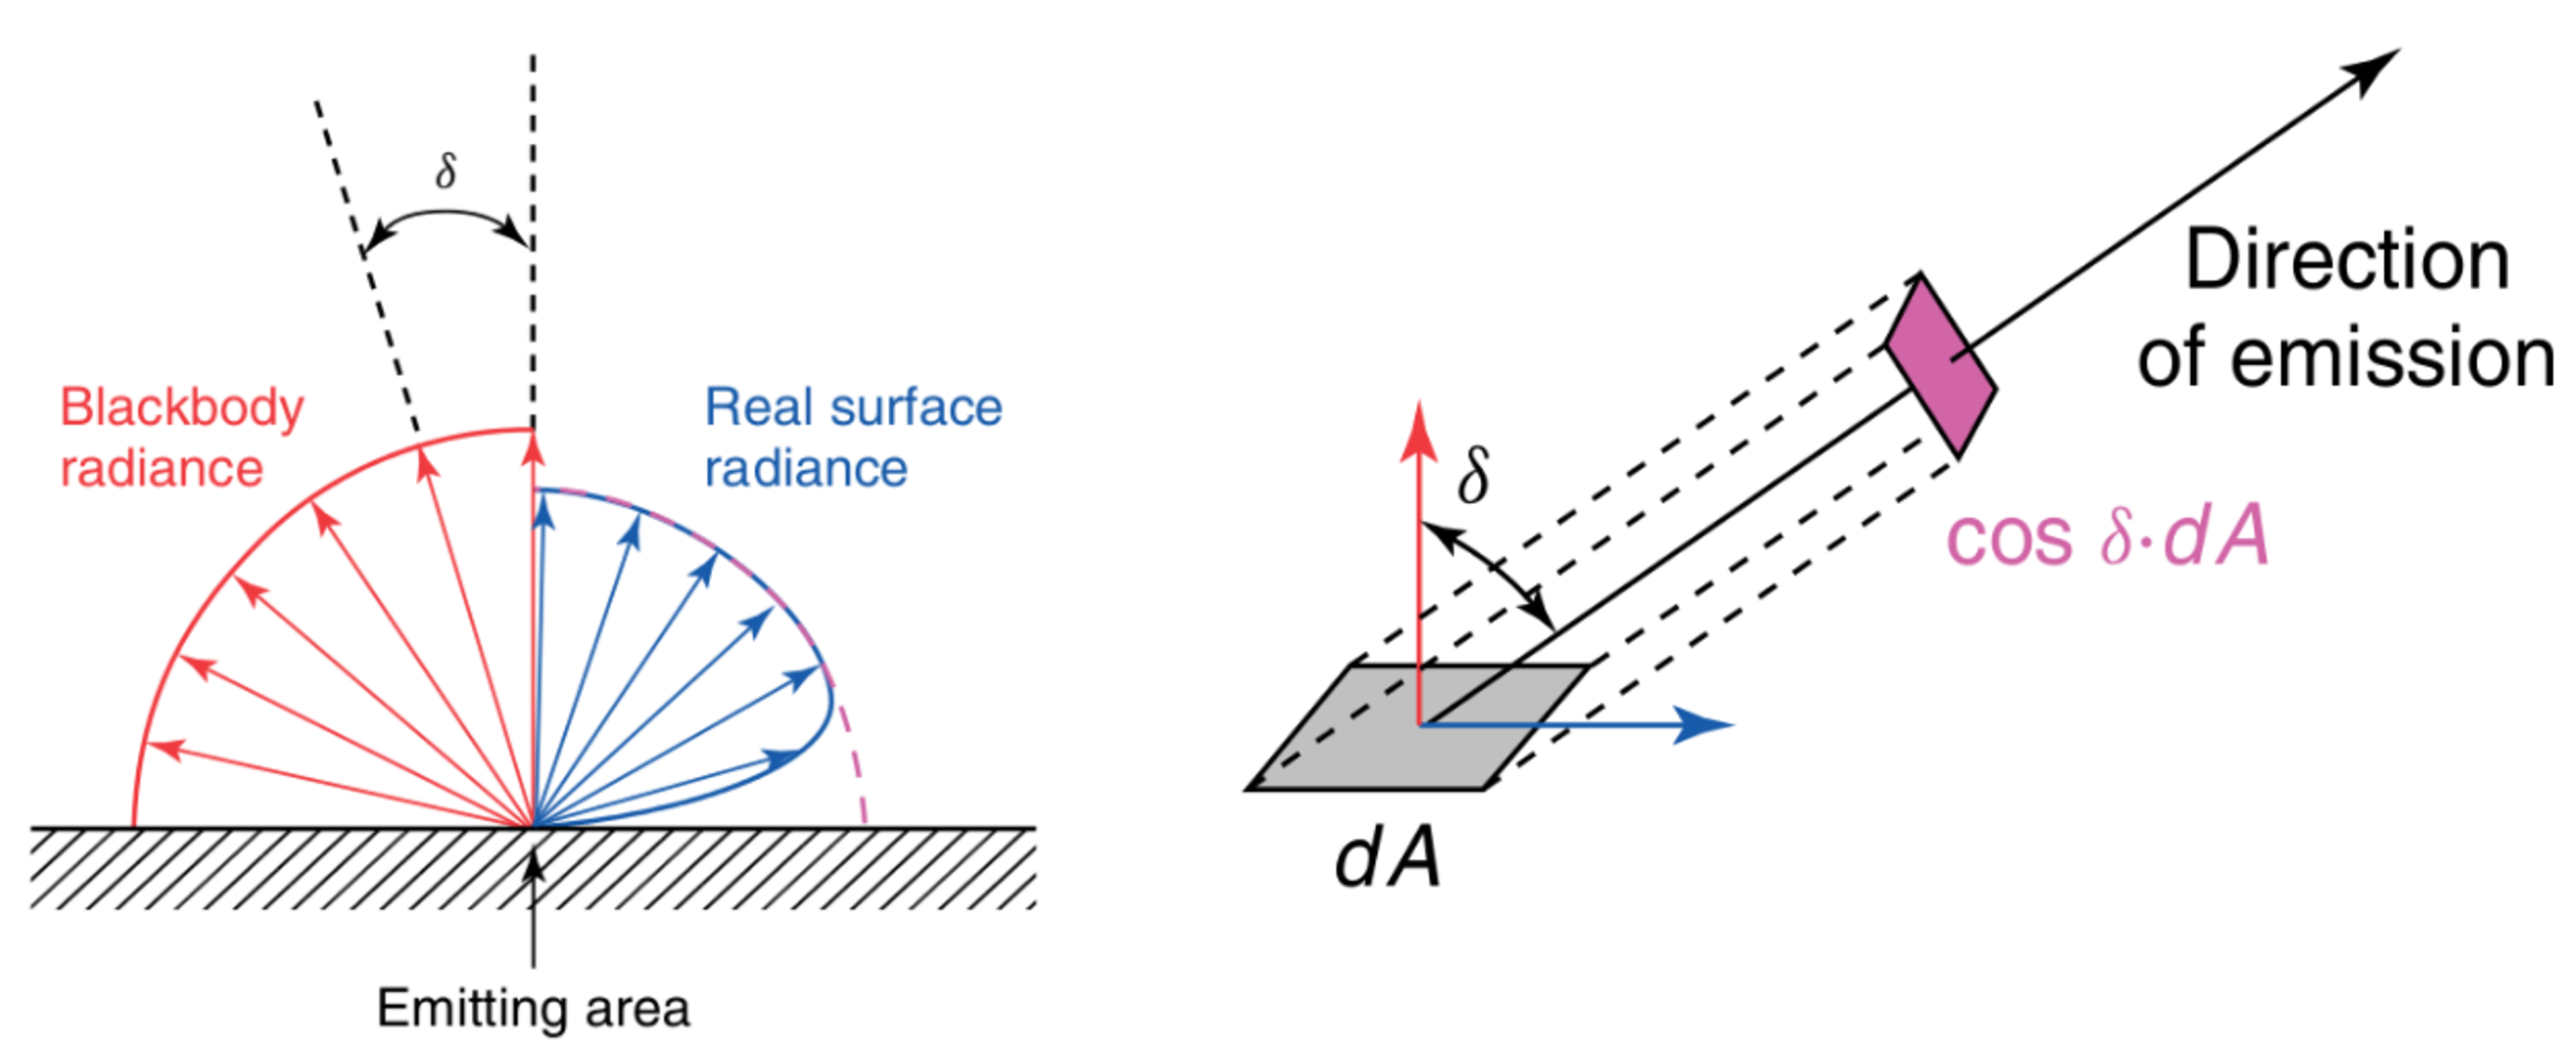
\includegraphics[scale=0.22]{Figures/Chapter03/AngularDistributionSchematics.pdf}
			\caption{Schematics of the angular dependence of the emissive power of a surface in relation to the blackbody}\label{fig3.2}
		\end{figure}
				
		Even though we can assume emissivity as a constant that only depends on the specific material of the surface under investigation, in general, it also depends on the viewing angle of the camera with respect to the normal of the surface. Blackbodies behave like perfect isotropically diffuse emitters, that is, for any surface emitting radiation, the radiance of the emitted radiation is independent of the direction into which it is emitted [8]. However, real surfaces, in addition to the lower emission rate (given by lower emissivity) also show angular dependence in the emissive power (Figure \ref{fig3.2} left).
		
		Usually, depending on the surface, the intensity of the emitted radiation might follow a cosine law with good approximation (Lambertian emitters). However, in general, this is not the case, and in most cases a study must be carried out to estimate the angular dependence of the emissivity [9, 10]. In order to determine whether this is a determining factor in our analysis, an angular study was performed using an aluminum rod filled with hot water placed in the same position as the Petal and, using a strip of high emissivity black tape along the rod's frontal face we were able to measure the variations in temperature due to the viewing angle (Figure \ref{fig3.3}).
				
		\begin{figure}[ht!]
			\centering
			\captionsetup{justification=centering,margin=2cm}
			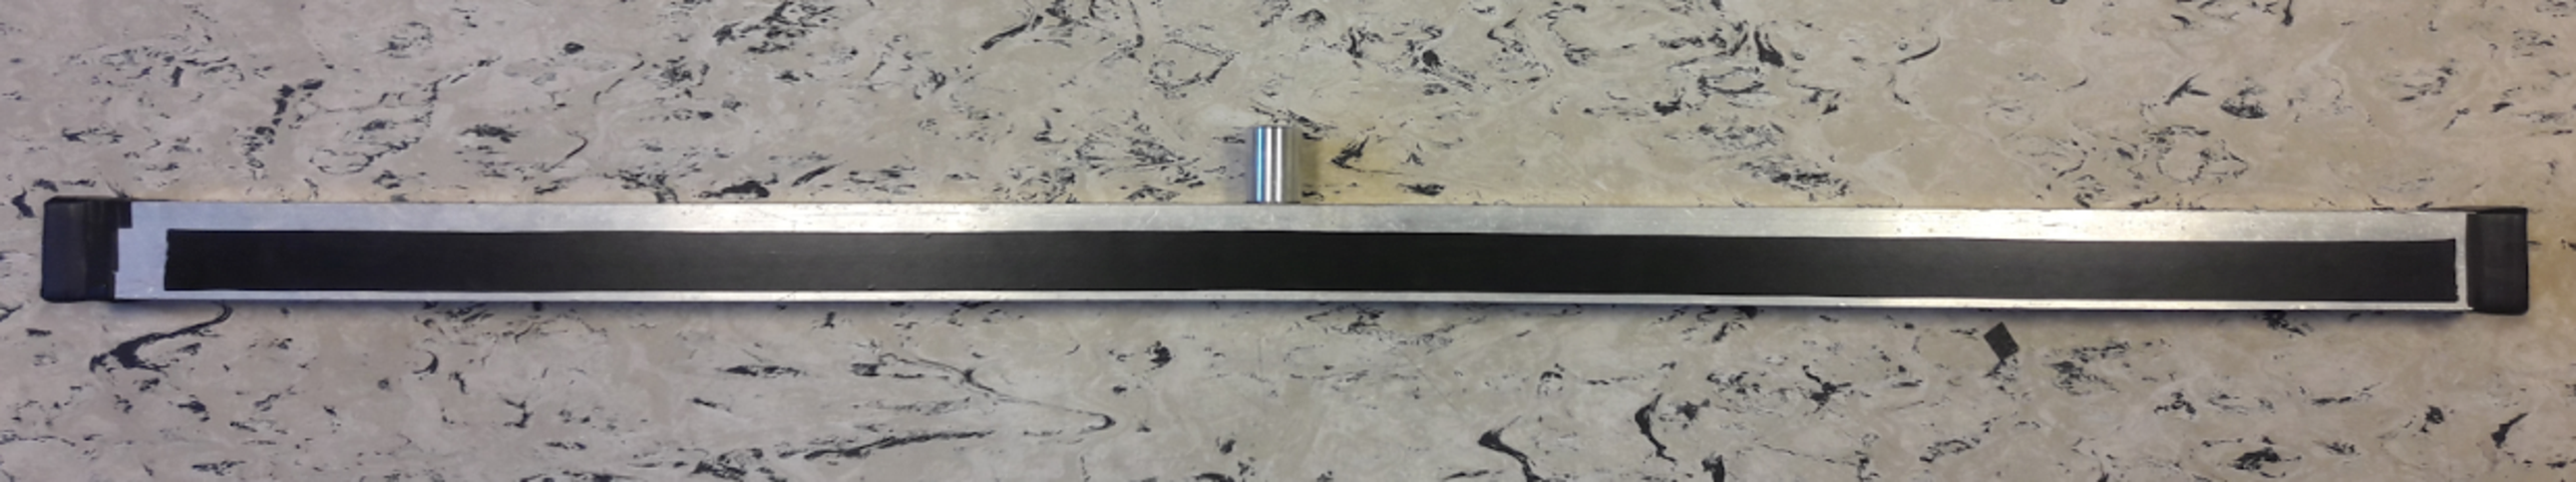
\includegraphics[scale=0.3]{Figures/Chapter03/AluminumRod.pdf}
			\caption{Aluminum rod used to study the angular dependence of emissivity.}\label{fig3.3}
		\end{figure}
		
		Of course, a combination of all the aforementioned factors leads to the small (but appreciable) differences between several materials in the image despite the fact that they are all at the same temperature. Figure \ref{fig3.4} shows an example of this effects in the emissive power perceived by the IR camera. This image is the ratio of the thermogram collected with the IR camera corresponding to the polished side of the Petal at room temperature (24.4 $^\circ C$ = 297.6 K) with no electronics powered on and no coolant flushed in and a thermogram where all the pixels have the same temperature of 297.6 K. This image clearly shows differences in temperatures among the different materials making visible the shape of the Petal itself. However, under ideal conditions, we shouldn't be able to distinguish any color variation since everything is supposed to be at the same temperature, that is, we should only see pixels with values of 1.
		
		\begin{figure}[ht!]
			\centering
			\captionsetup{justification=centering,margin=2cm}
			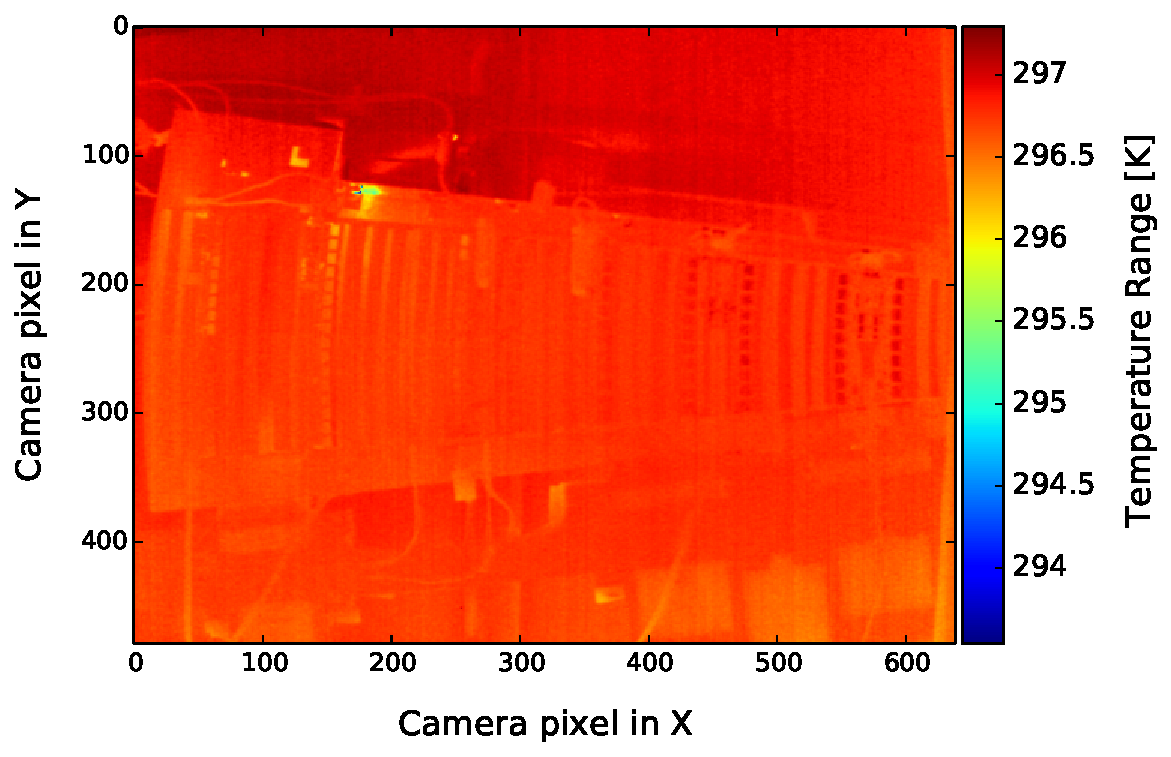
\includegraphics[scale=0.5]{Figures/Chapter03/thermo_Temp_201708091701_avg.pdf}
			\caption{Ratio thermogram of the Petal at room temperature. If the IR camera were 100\% accurate we should see all pixels with a ratio value of 1.}\label{fig3.4}
		\end{figure}
		
		In order to obtain an IR image as accurate as possible we must account (correct) for as many of this factors as we can. In the following sections we discuss in more detail the procedures used to estimate the contribution of the most important ones: emissivity, apparent reflected temperature and spectral response function of the camera.
	
		\subsection{Apparent reflected temperature estimation.}\label{section3.1.1}
		
			In order to correctly estimate the emissivity of any surface it is very important to determine first the surface apparent reflected temperature. This is crucial, especially for low emissivity materials where the most important contribution is in fact the reflected radiation.
			A simple method can be used to determine the apparent reflected temperature. This method is described as follows:
			
			\begin{enumerate}[label={\arabic*)}]
				\item Place a piece of crumpled and re-flattened aluminium foil in the same position of the object to be measured.
				\item Set the IR camera emissivity control to 1.00 and distance to 0 m.
				\item Point the IR camera to the target and select a region of interest (ROI).
				\item Measure the apparent surface temperature of the ROI.
				\item Take the measured value as the apparent reflected temperature.
			\end{enumerate}
			
			Aluminum foil has very low emissivity ($\sim$ 0.04) and therefore we are certain that almost all IR radiation coming from the surface is reflected from other sources. The emissivity and distances settings of 1.00 and 0 m respectively are just telling the camera that record everything without applying any further correction. The crumpling is done to allow reflections from several directions, for this reason the ROI selected should be as wide as possible since this effect must be averaged out to obtain an accurate estimate of the apparent reflected temperature.
	
		\subsection{Emissivity estimation. Viewing angle influence.}\label{section3.1.2}
		
			A good illustration of the effect of emissivity in the measurement of the real temperature of a surface is presented in Figure \ref{fig3.5}. This corresponds to the so called Leslie’s Cube. Even though this cube is filled with hot water and all the faces are at the same temperature we can see a huge difference in the temperature measured by the IR camera. This is due to the difference in emissivity of the two front faces. One is painted with a high emissivity black (could be any color) paint and therefore the apparent temperature is closer to the real temperature of the water, while the other face is very reflective (low emissivity) and the apparent temperature is almost entirely due to the reflected component.
			As the main source of discrepancies comes from the differences in emissivity, this is very often the starting point for IR image calibration. Almost all IR cameras can be set to a certain value of emissivity (usually set to 1 by default). If we knew the emissivity value of certain surface we could then enter that value into the IR camera software and the apparent temperature would be close to the real temperature. This is what we would call a “direct” emissivity correction method. It is of course the most simple but also the most uncommon way to correct an IR image for more complicated quantitative studies. On one side, we usually don’t know beforehand the emissivity value of the surface we want to measure and, on the other side, this method would only give us the correct temperature on the surface of known emissivity.
			
			\begin{figure}[ht!]
				\centering
				\captionsetup{justification=centering,margin=2cm}
				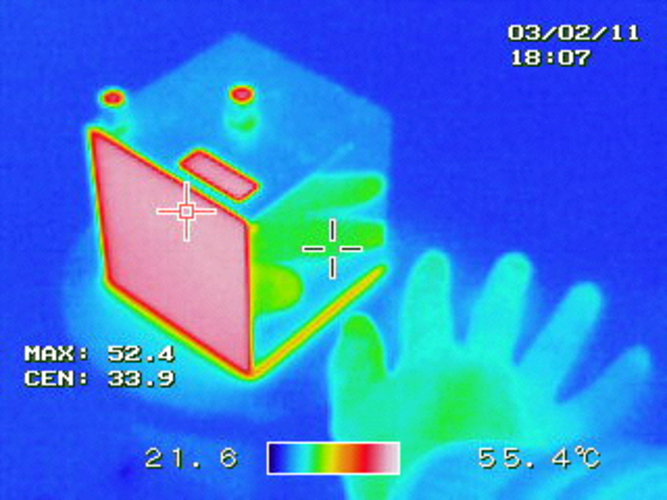
\includegraphics[scale=0.6]{Figures/Chapter03/LesliesCube.pdf}
				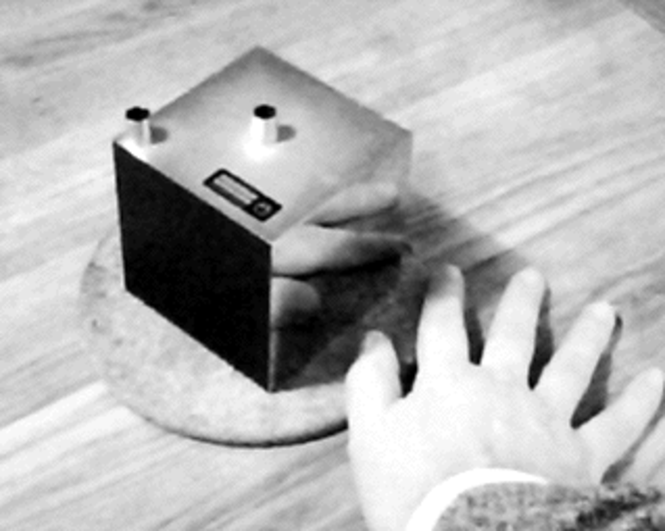
\includegraphics[scale=0.57]{Figures/Chapter03/LesliesCube2.pdf}
				\caption{Infrared (Left) and visible (Right) images of a Leslie's cube. The cube is filled with hot water and all the faces are at the same temperature. However,  one of the faces is coated with a high emissivity paint (black) and the other has been polished (low emissivity).}\label{fig3.5}
			\end{figure}	
			
			For the Petal's thermal study an equally effective alternative was used: the silicon surface on both sides of the Petal were coated with high emissivity black tape (Figure \ref{fig3.6}). The black tape used has an emissivity of 95\% and therefore the coated surface will behave almost like a blackbody. This is known as the “coating” method and, as the name indicates, consists in coating the surface of interest with a material of known emissivity (ussually high emissivity) and use the direct correction method on the coated surface. 
			For our black taped Petal (“zebra”), setting the IR camera emissivity to the emissivity of the black tape we can measure an apparent temperature very close to the real temperature assuming that both the surface of interest and the black tape on top of it have reached a steady state at the same temperature. Using the IRBIS software a set of over 560 measurement markers (ROIs) were created all over the black tape strips to create a sort of map of temperatures. With this method we could perform relatively accurate temperature measurements on the Petal's silicon surface to be able to compare with FEA simulations (See chapter 4). However, as it can be seen from the picture, we had to cover almost entirely the silicon surface, which would be unacceptable during production stages for quality control. Furthermore, a set of markers was also created for the silicon surface right next to the corresponding black tape marker to study the emissivity behaviour of the silicon using the black tape markers readings as the “real” temperature values.
			
			\bigskip
			There are also some other ways to calculate the emissivity of a surface. One of them consists in estimating the surface’s emissivity by using an alternative temperature measurement as reference. With that purpose, the following method can be used [11, 12]:	
			
			\begin{enumerate}[label={\arabic*)}]
				\item Measure the surface temperature by an alternative method (thermocouple, known emissivity coating).
				\item Set the necessary measurement parameters in the IR camera software and the emissivity to 1.
				\item Point the IR camera to the target and select a region of interest (ROI).
				\item Modify the value of emissivity in the camera software until the apparent temperature in the selected ROI equals the one measured with the alternative method. This is the emissivity of the target surface.
				\item Repeat steps 2) to 4) as many times as necessary to minimize the measurement uncertainty.
			\end{enumerate}	
			
			\begin{figure}[ht!]
				\centering
				\captionsetup{justification=centering,margin=2cm}
				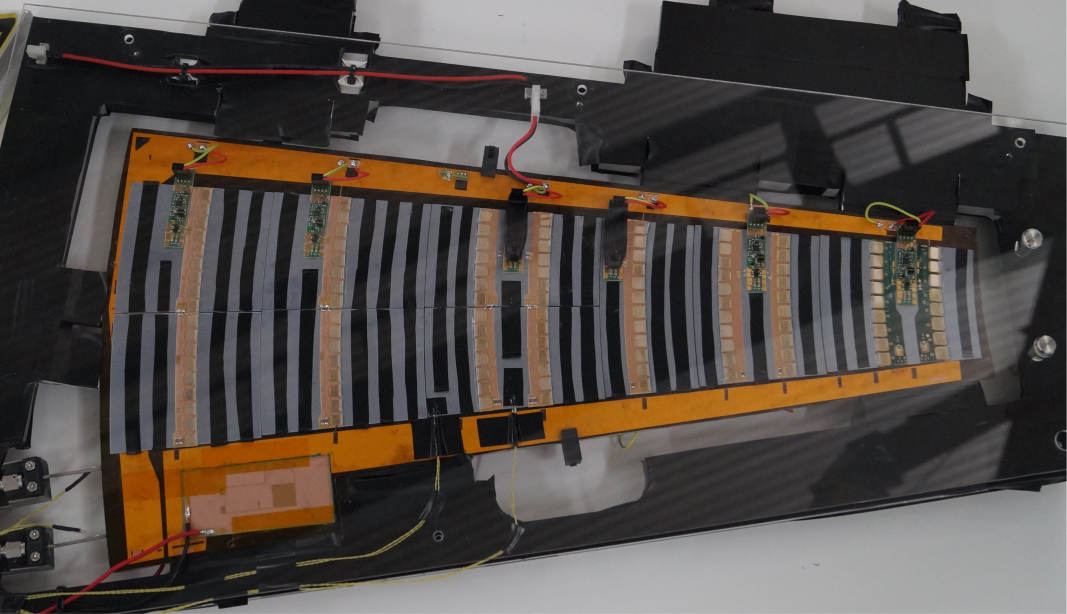
\includegraphics[scale=0.45]{Figures/Chapter03/ZebraPetal.pdf}
				\caption{Unpolished side of the “Zebra” Petal covered with stripes of black electrical tape of high emissivity.}\label{fig3.6}
			\end{figure}
			
			Using this approach a “global” IR image emissivity correction can be applied to get temperature values close to the real ones in the silicon surface. However, as mentioned before, this will only show accurate readings in those areas of the image where the surface of estimated emissivity is. The rest of the elements in the image that have different emissivity values might appear to have a complete different temperature of what they actually have. Even so, if we are not interested in the whole picture but just in one particular material in it, this simple method can be very useful. The problems begin when the surface of interest has relatively low emissivity. In such cases temperature estimation may not be very accurate because low emissivities are hard to estimate and small changes in its value can lead to large variations in the temperature measurements [13, 14]. In other words, the lower the emissivity of the surface, the bigger the systematic uncertainty associated with it.
			Another approach consists in using a “relative” method exploiting the Equation \ref{eq3.9}. Lets imagine that we have two surfaces at the same temperature, then, if we apply Equation \ref{eq3.9} on the one that we know the emissivity value (e.g. black tape) and on the one we want to estimate it from (e.g. silicon surface) then we obtain:
			
			\begin{equation}\label{eq3.12}
				N^{BT}_{meas}(T_{BT})= R \cdot \bar{\varepsilon}_{BT} \cdot I_{1}(T_{BT}) + R \cdot [1- \bar{\varepsilon}_{BT}] \cdot I_{2}(T_{r})
			\end{equation}
			
			\begin{equation}\label{eq3.13}
				N^{Si}_{meas}(T_{BT})= R \cdot \bar{\varepsilon}_{Si} \cdot I_{1}(T_{BT}) + R \cdot [1- \bar{\varepsilon}_{Si}] \cdot I_{2}(T_{r})
			\end{equation}
			
			Note that as the “real” temperature we have selected the apparent temperature of the black tape ($T_{BT}$). We can do so since the black tape has high emissivity. Naturally we know that $N^{BT}_{meas}(T_{BT}) \neq N^{Si}_{meas}(T_{BT})$, however, we can use a small trick here: as the black tape has high emissivity, if we replace $T_{BT}$ in Equation \ref{eq3.12} with the silicon apparent temperature ($T_{Si}$) then $N^{BT}_{meas}(T_{Si}) \equiv N^{Si}_{meas}(T_{BT})$ and after rearrange terms we obtain:
			
			\begin{equation}\label{eq3.14}
				\bar{\varepsilon}_{Si} = \bar{\varepsilon}_{BT} \cdot \frac{I_{1}(T_{Si}) - I_{2}(T_{r})}{I_{1}(T_{BT}) - I_{2}(T_{r})}
			\end{equation}
			
			Note that this expression is invalid if the silicon surface is considerably transmissive, since we have neglected transmissivity for deriving Equation \ref{eq3.9}, and when the real temperature ($T_{BT}$) is close to $T_{r}$ in which case Equation \ref{eq3.14} is undefined.
		
		\subsection{IR camera spectral response.}\label{section3.1.3}
			
			From Equation \ref{eq3.9} it can be seen that if we can accurately estimate emissivity, apparent reflected temperature and the IR camera spectral response function we should be able then to obtain the real temperature of the object for any given output of the camera ($N_{meas}$). 
			In order to obtain the $R$ factor we can simply take the emissive power measurements of a surface of known emissivity, the real temperature and the apparent reflected temperature and then use the same Equation \ref{eq3.9} to derive the $R$ scale factor. As this factor only depends on the IR camera, it can be used later on in the analysis as long as we don’t use a different camera.
			To obtain the scale factor for our analysis we used an aluminum bucket which we filled with hot water and recorded the IR power density on several points of the surface (always at the same depth) coated with black tape as the water temperature went down to test the temperature independence of the results (Figure \ref{fig3.7}). 
						
			\begin{figure}[H]
				\centering
				\captionsetup{justification=centering,margin=2cm}
				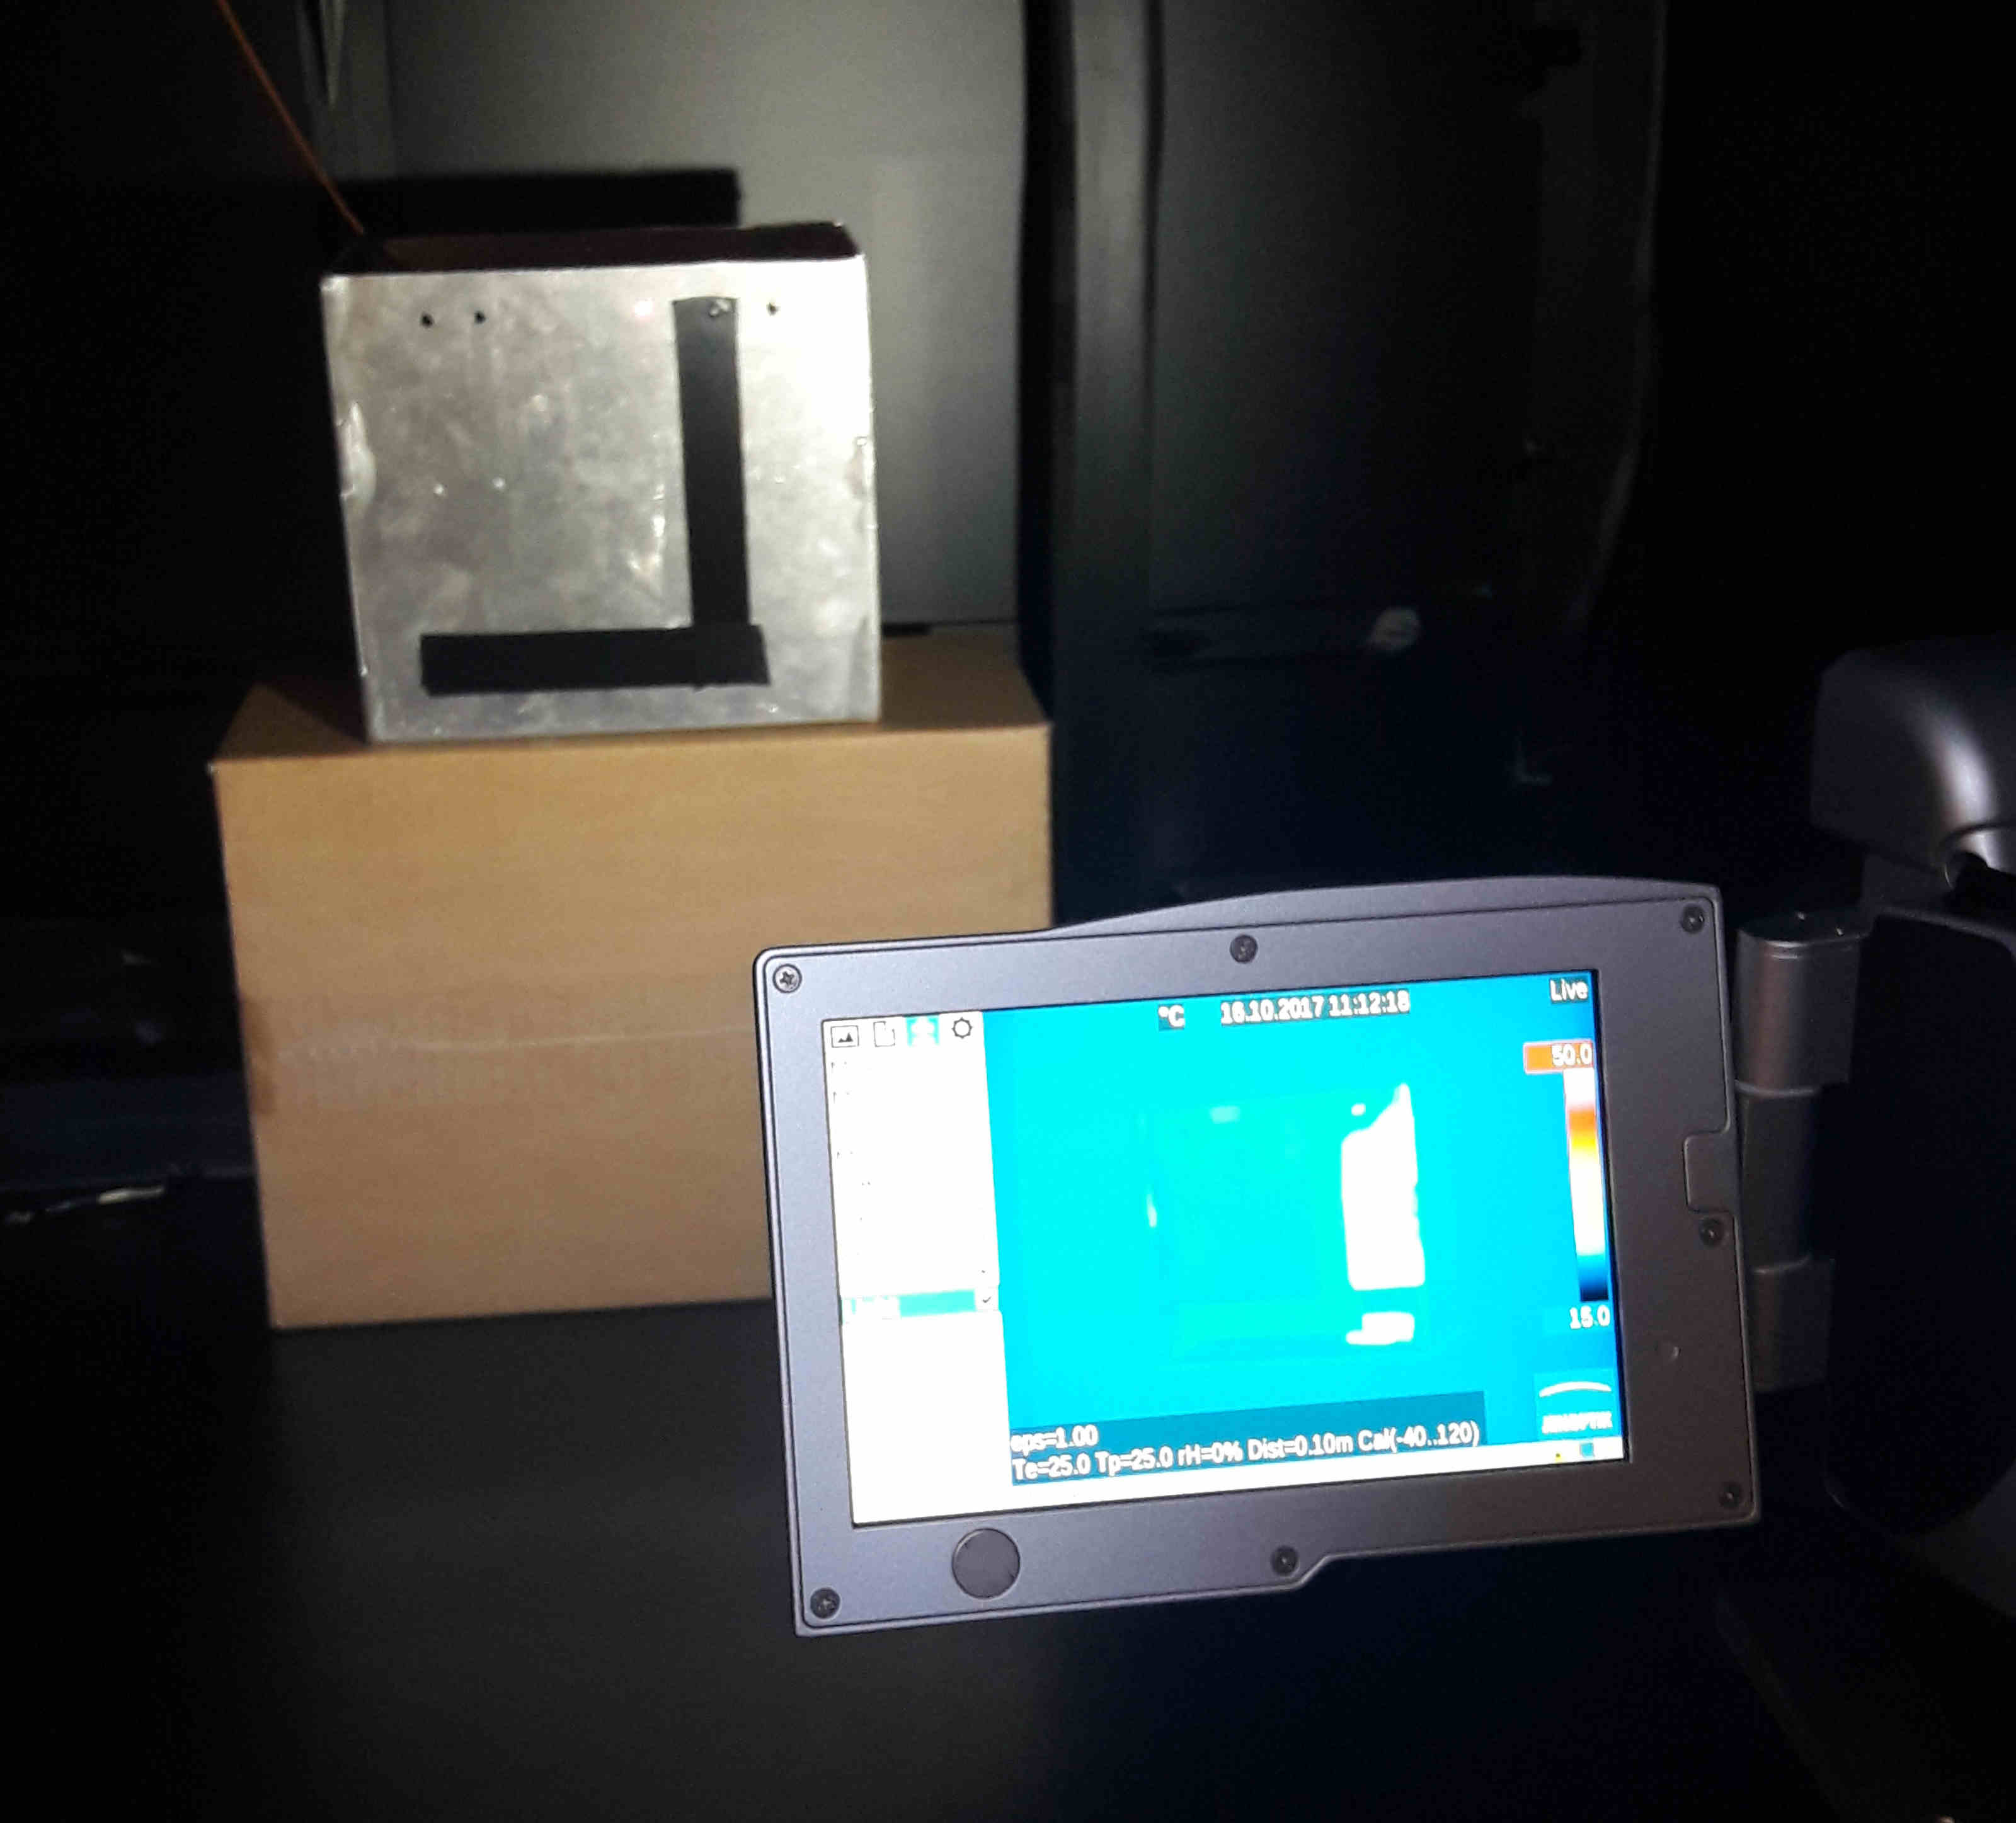
\includegraphics[scale=0.12]{Figures/Chapter03/CameraAndBucket.pdf}
				\caption{Experimental setup to calculate the IR camera spectral response function. Measurements were performed placing 8 measurement markers along the horizontal black tape in the camera IRBIS software.}\label{fig3.7}
			\end{figure}	
		
		
	